\documentclass[12pt]{article}
\usepackage{graphicx}
\usepackage{geometry}
\usepackage{hyperref}
\usepackage{amssymb}
\graphicspath{ {./images/} }
\geometry{a4paper,left=20mm,top=20mm,}


\begin{document}
\title{
    
\includegraphics[scale=0.125]{logo.jpg}\\
    \vspace*{6cm}
    Haptic Sensor Integrated Robot Arm\\
    \vspace*{6cm}}

\author{Kanishk Navale\\Student Assistant-Haptic Intelligence\\Max-Planck-Institut für Intelligente Systeme\\70569 Stuttgart - DE}
\date{June 14, 2021}

\maketitle
\pagebreak

\tableofcontents
\listoffigures
\pagebreak

\section{Robot \& Physics Solver}
    \subsection{Robot: `nyu\_finger'}
        The robot is constructed in accordance with the \href{https://github.com/open-dynamic-robot-initiative}{Open Dynamic Robot Initiative}.
        The \href{https://github.com/open-dynamic-robot-initiative/nyu_finger}{`nyu\_finger'} is one of the robots.
        The initial robot driver \cite{robot_drivers} is developed by Julian Viereck licensed under BSD 3-Clause License with Copyright(c) 2020 Max Planck Gesellschaft, New York University.
        The below image emphasis on the build of the robot along with its kinematic description.
        \begin{figure}[h]
            \centering
            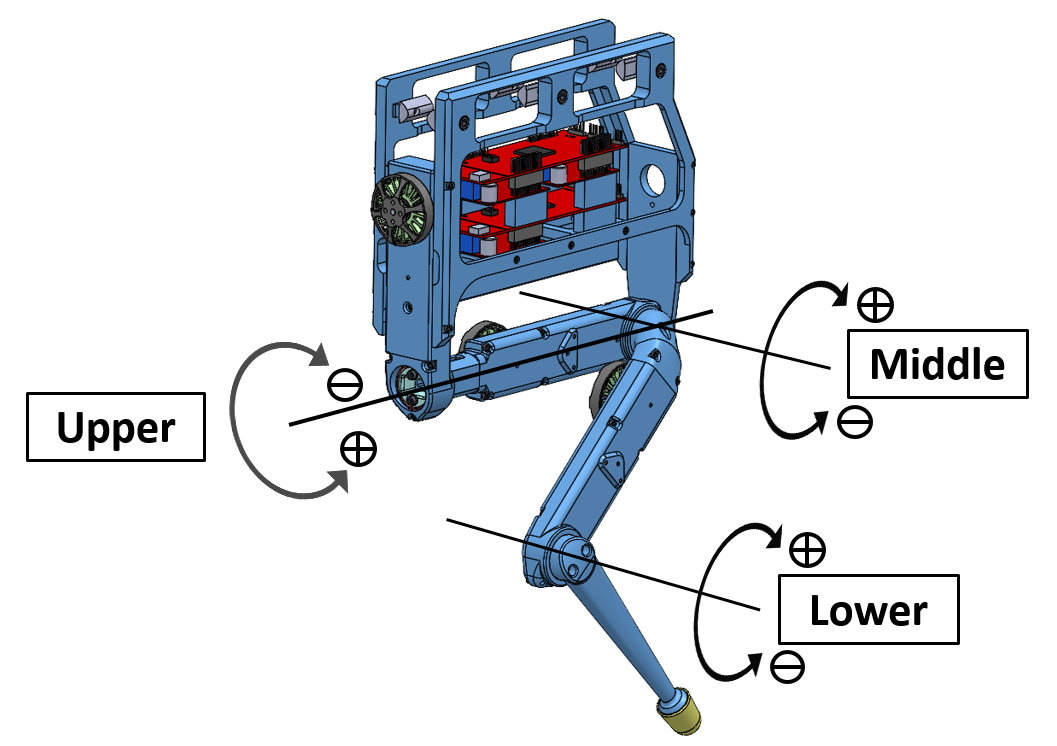
\includegraphics[scale=0.5]{finger_edu_joint_labels_1.png}
            \caption{Illustration of the manipulator.}
        \end{figure}

    \subsection{Physics Solver: Pinocchio}
        ``Pinocchio instantiates the state-of-the-art Rigid Body Algorithms for poly-articulated systems based on revisited Roy Featherstone's algorithms. 
        Besides, Pinocchio provides the analytical derivatives of the main Rigid-Body Algorithms like the Recursive Newton-Euler Algorithm or the Articulated-Body Algorithm."\\
        source: \href{https://github.com/stack-of-tasks/pinocchio}{stack-of-tasks/pinocchio} \cite{pinocchio}\\

        The code library contains limited detailed description for some functions. This can cause few issues during the implementation of the robot functionalities.
        \pagebreak

\section{Kinematics Solver}
    The Pinocchio library constructs the robot kinematic-tree using the .urdf files in the 'nyu\_finger' repository. 
    The library comes with several functionalities solving the same tasks. The robot needs a reference frame to compute the transformation. 
    This is solved by invoking a visualizer \& approximating frames used by the robot. The correct kinematic function is found by trying out all the similar functions \& counter-checking it mathematically.   

    \subsection{Visualizers}
        \subsubsection{MeshCat}
            The `MeshCat Visualizer' comes equipped with the Pinocchio. This visualizer runs in a web browser. 
            As the robot needs the `sudo' privileges in the Linux machine to run the visualizer could not run in a web browser anymore due to the limitations of the visualizer.
            \begin{figure}[h]
                \centering
                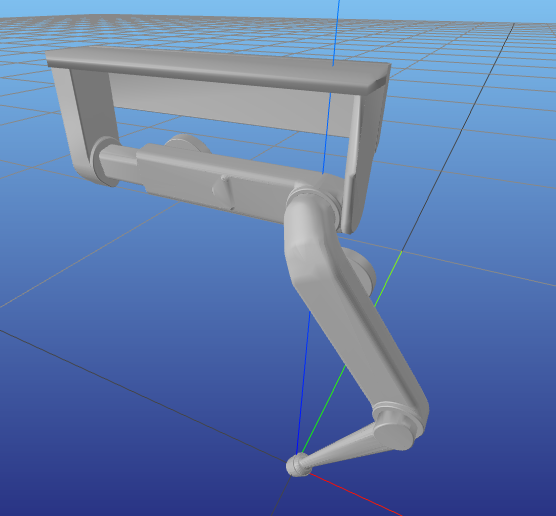
\includegraphics[scale=0.27]{meshcat.png}
                \caption{Rendering in `MeshCat Visualizer'.}
            \end{figure}

        \subsubsection{NYUFingerSimulator}
            The `NYUFingerSimulator' is used to simulate the robot. With a few code tweaks the simulator is turned into visualizer 
            solving the issue with the previous visualizer.
            \begin{figure}[h]
                \centering
                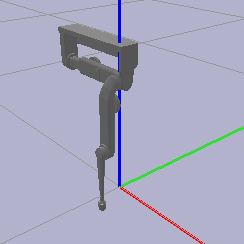
\includegraphics[scale=0.6]{simulator.png}
                \caption{Description of the simulator.}
            \end{figure}

        \subsection{Inverse Kinematics}
            The inverse kinematics for the robot is implemented based on optimization. The algorithm in the below figure 
            explains the optimization and method in much detail.
            \begin{figure}[h]
                \centering
                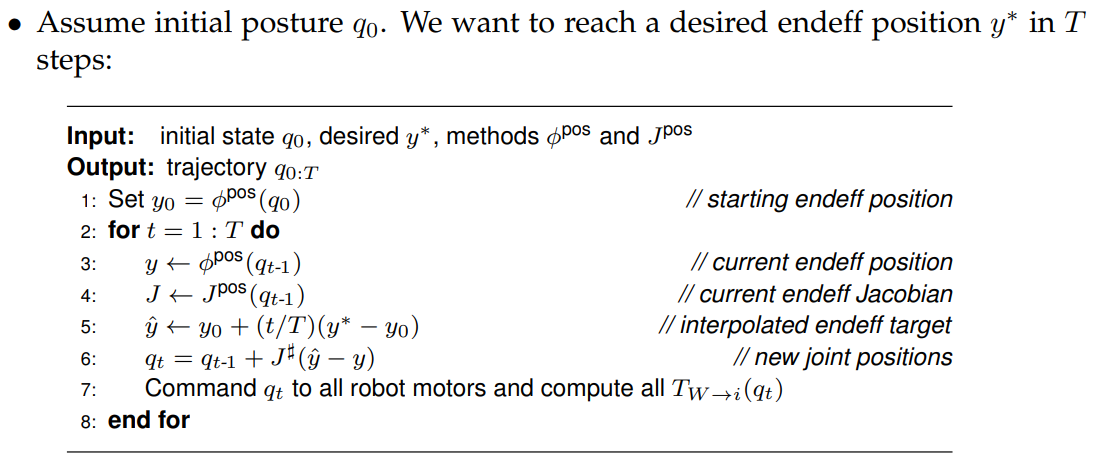
\includegraphics[scale=0.35]{IK.png}
                \caption{Description of the Inverse Kinematics solver.}
            \end{figure}\\
            source: \href{https://www.user.tu-berlin.de/mtoussai//teaching/Lecture-Robotics.pdf}{Introduction to Robotics - Marc Toussaint}
        
        \subsection{Robot Teleoperation using Keyboard}
            \href{https://www.pygame.org/docs/}{`pygame'} is a pyhton3 library for developing games. 
            Moreover, it provides a realtime interface modules for the Keyboard. The event handlers for the Keyboard is much stable with it.
            The inverse kinematics is mapped to certain keys moving the robot relatively in the cartesian space with fixed step distances. 
            This functionality is tested in the simulator. In the upcoming phase, the keyboard will be replaced by the haptic sensor.
            The sensor is capable to move the robot in the cartesian space with varying velocity or force.

\section{Dynamics Solver}
    \subsection{Inverse Dynamics Compensation}
        As the robot actuators are BLDC motors they are not equipped with the brakes. 
        The moment the robot stops receiving joint commands the robot loses it's configuration due to gravity.
        To solve this, Inverse Dynamic terms like Gravity, Corrolis, Centrifugal and Inertial Compensations are used to compute joint torques to preserve the robot stance.
        The joint commands is issued at an rate of 60Hz.

    \subsection{Position \& Velocity Control}
        For controlling the robot's position and velocity seperate PID loops are implemented. 
        As per the experiments PID based controller is not yielding desired results with varying steady state error inspite having individual gain vectors for each actuators.
        The motor driver expects a joint command every 1ms posing an issue in realtime code performance.
        Presently, PID based controller is being ported to LQR based controller for better results.  

\section{Robot Class}
    The robot class implements all the functionalities into an object. 
    There are few tasks like Inverse Dynamics Compensations \& Updating the simulator running in the background.
    Overview and brief description of robot capabilites are as follows,

    \begin{enumerate}
        \item Simulator,\\
        Reads the positions of robot joints in realtime \& updates the visualizer at rate of 60Hz.

        \item Inverse Dynamic Compensations,\\
        Preserves the robot stance against the gravity \& external forces by issuing compensating torques at the rate of 1000Hz.
        
        \item Teleoperation,\\
        If enabled, the robot can be moved using keyboard. The `pygame' runs at an rate of 1Hz.

        \item Reading Haptic Sensor,\\
        The robot reads the sensor at the rate of 1000Hz.

        \item Point-to-Point Motion Functionality,\\
        This functionality is extended from the Inverse Kinematics Solver. The robot can between two or more points in the cartesian space in Joint or Linear Travesial Mode.
        It also 3D plots the position of the TCP if enabled.
    \end{enumerate}

    \subsection{Handling Relative Encoders}
        The actuators is equipped with the relative encoders meaning during power cycle the actuator's states are lost.
        For time being, the robot is crudely positioned at an zero pose and the offsets are biased.
        This procedure sometimes causes a mismatch in computing terms for robot dynamics.
        Another way to turn them into absolute encoders is to implement a CMOS at a hardware level.

    \subsection{Pipelining Model \& .urdf File Updates}
        As the .urdf file encompasses dynamic parameters like as mass, interia etc. any changes in the hardware of the robot needs calibration in the code side.
        The better way to get around this is to build an pipeline which translates 3D model to .urdf files to hardware changes.
        The pipeline can be constructed using services in the project management systems.
        This eliminates the calibration procedure in the codebase everytime when systems engineering components are added to robots.  
    \pagebreak

\section{Haptic Sensor}
    The sensor is based of capacitance sensor array of $\mathbb{R}^{n \times n}$. 
    The robot reads 21 channels of data from the sensor using serial port.
    The serial port is dynamically searched by the robot.
    The data can be parallely visualized in chart \& matrix form as described by the following image,
    \begin{figure}[h]
        \centering
        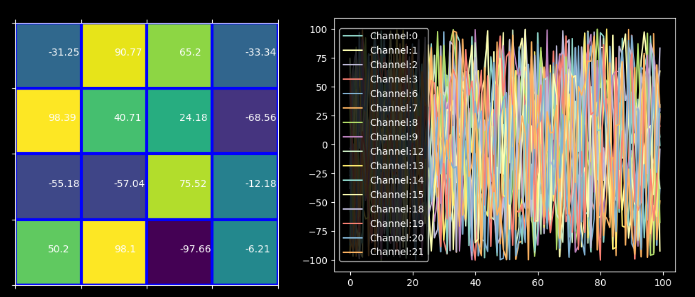
\includegraphics[scale=0.65]{sensor_monitor.png}
        \caption{Illustration of the sensor monitoring.}
    \end{figure}

\section{Upcoming Tasks}
    \begin{enumerate}
        \item Test the LQR Controller.
        \item Implement Impedence Controller working alonside with the sensor.
        \item Improve code performance.
        \item Implement CMOS based Encoders. (To be discussed)
        \item Converting Sensor reading into force vector of $\mathbb{R}^3$
    \end{enumerate}

    \bibliographystyle{unsrt}
    \bibliography{localbibliograpghy.bib}
   
\end{document}